\section{Average Vehicle Speed}
\label{sec:Results_MeanSpeed}

Table~\ref{tab:MeanSpeed} and Figures~\ref{fig:MeanSpeed_2077}–\ref{fig:MeanSpeed_3462} report the mean cruise speed of the platoon as a function of \ac{mpr}. The three control strategies, Standard, \ac{eco-glosa} and \ac{flow-glosa}, are compared under both emission models (HBEFA4 and PHEMLIGHT5) at three critical demand levels. A careful examination of the data yields six principal insights.

\subparagraph*{1. Systematic impact of \ac{mpr} on \ac{eco-glosa}.}
Across \emph{all} volumes, \ac{eco-glosa} shows a monotonic speed decrease as \ac{mpr} increases. For example, at the lightest load of $69\,\mathrm{veh/h}$, the HBEFA4 mean speed drops from $13.34\,\mathrm{m/s}$ (Standard) to $13.01\,\mathrm{m/s}$ at $100\,\%$ \ac{mpr} ($\downarrow 2.5\,\%$). The reduction accelerates with demand: at $2077\,\mathrm{veh/h}$, the decrease is $0.44\,\mathrm{m/s}$ ($\downarrow 3.5\,\%$) by $40\,\%$ \ac{mpr}, while at $2769\,\mathrm{veh/h}$ it becomes catastrophic, falling from $11.94\,\mathrm{m/s}$ to $2.57\,\mathrm{m/s}$ ($\downarrow 79\,\%$) by $90\,\%$ \ac{mpr} under PHEMlight5 (Figure~\ref{fig:MeanSpeed_PHEM_2769}). This monotonic decline is, for example, illustrated in Figures~\ref{fig:MeanSpeed_HBEFA4_2077} and~\ref{fig:MeanSpeed_PHEM_2077}.

\subparagraph*{2. Flow stability and jam resolution of \ac{flow-glosa}.}
\ac{flow-glosa} maintains near-Standard speeds up to $2769\,\mathrm{veh/h}$, and under full saturation ($3462\,\mathrm{veh/h}$) it dissolves the queue once penetration exceeds approximately $80\%$. The mean speed increases from $\mathbf{3.86\,\mathrm{m/s}}$ (Standard, 0\% \ac{mpr}) to $4.16\,\mathrm{m/s}$ at $50\%$ \ac{mpr} and ultimately reaches $\mathbf{12.18\,\mathrm{m/s}}$ at $100\%$ \ac{mpr}. This behaviour demonstrates that \ac{flow-glosa} can actively resolve gridlock and restore free-flow speeds when a sufficient share of vehicles conforms to its advisory. The jam-dissolving capability is evident in Figures~\ref{fig:MeanSpeed_HBEFA4_3462} and~\ref{fig:MeanSpeed_PHEM_3462}.  


\subparagraph*{3. Emission-model sensitivity.}
PHEMlight5 consistently produces lower speeds than HBEFA4 at the same \ac{mpr} and demand level. The difference is modest at low demand (approximately $0.1\,\mathrm{m/s}$ for $69$--$346\,\mathrm{veh/h}$) but widens dramatically in congestion. At $2769\,\mathrm{veh/h}$ and $30\,\%$ \ac{mpr}, PHEMlight5--\ac{eco-glosa} already drops to $3.17\,\mathrm{m/s}$ versus $7.32\,\mathrm{m/s}$ for HBEFA4, a $57\,\%$ gap. This reflects the higher temporal resolution and the non-linear fuel--speed polynomial in PHEMlight5: it penalises short bursts of high engine power more strongly, which prompts earlier decelerations and thus longer queuing times. The widening gap between HBEFA4 and PHEMlight5 under congestion is visible in Figures~\ref{fig:MeanSpeed_HBEFA4_2769} and~\ref{fig:MeanSpeed_PHEM_2769}.

\subparagraph*{4. Jam-onset thresholds.}
Under the conventional jam criterion of around $v \leq 4\,\mathrm{m/s}$ in urban areas, Table~\ref{tab:MeanSpeed} reveals discrete breakpoints for the \ac{eco-glosa}. In the PHEMlight5 case, a jam forms at $10$--$20\,\%$ \ac{mpr} for $2769\,\mathrm{veh/h}$ and at the first non-zero \ac{mpr} for $3462\,\mathrm{veh/h}$. HBEFA4 postpones the jam onset by roughly one \ac{mpr} decade: $30$--$50\,\%$ at $2769\,\mathrm{veh/h}$. The staggered thresholds underscore the importance of the emission-model choice when extrapolating eco-driving benefits to congested corridors. The onset of jam (v\,$\le4\,\mathrm{m/s}$) corresponds to the inflection points in Figures~\ref{fig:MeanSpeed_HBEFA4_2769} and~\ref{fig:MeanSpeed_PHEM_2769}.

\subparagraph*{5. Residual overshoot at low demand.}
At sub-saturated volumes ($69$--$1385\,\mathrm{veh/h}$), \ac{eco-glosa} occasionally overshoots Standard by up to $0.04\,\mathrm{m/s}$ at $10\,\%$ \ac{mpr}. The effect, most visible in HBEFA4, originates from the algorithm's \enquote{anticipatory glide} that smooths minor stop-and-go waves, thereby shortening braking phases and slightly increasing the arithmetic mean of cruise speed. However, as soon as \ac{mpr} exceeds approximately $20\,\%$, the fuel-saving bias dominates and the curve bends downward. The slight overshoot at low demand (10\,\% \ac{mpr}) is observable in Figures~\ref{fig:MeanSpeed_HBEFA4_2077} and~\ref{fig:MeanSpeed_PHEM_2077}.

\subparagraph*{6. Progressive speed gains under \ac{flow-glosa}.}
As \ac{mpr} increases, \ac{flow-glosa} delivers measurable speed improvements even below saturation. At low demand ($69\,\mathrm{veh/h}$), HBEFA4–\ac{flow-glosa} speeds climb from $\mathbf{13.34}$ to $13.88\,\mathrm{m/s}$ ($+4.1\,\%$) by $90\,\%$ \ac{mpr}. At medium demand ($1385\,\mathrm{veh/h}$), the mean speed rises from $\mathbf{12.84}$ to $13.07\,\mathrm{m/s}$ ($+1.8\,\%$) at $100\,\%$ penetration. Even at high demand ($2769\,\mathrm{veh/h}$), it increases from $\mathbf{11.94}$ to $12.55\,\mathrm{m/s}$ ($+5.1\,\%$) at $100\,\%$ \ac{mpr}. These consistent gains underscore \ac{flow-glosa}’s capacity to smooth stop-and-go waves and improve throughput across light, moderate, and heavy traffic regimes. The progressive uplift with increasing penetration is shown by the upward slopes in Figures~\ref{fig:MeanSpeed_HBEFA4_2077}, \ref{fig:MeanSpeed_HBEFA4_2769}, and \ref{fig:MeanSpeed_HBEFA4_3462} (and similarly for PHEMLIGHT5 in Figures~\ref{fig:MeanSpeed_PHEM_2077}, \ref{fig:MeanSpeed_PHEM_2769}, \ref{fig:MeanSpeed_PHEM_3462}).

\begin{figure}[htb]
  \centering
  \begin{subfigure}[b]{0.49\textwidth}
    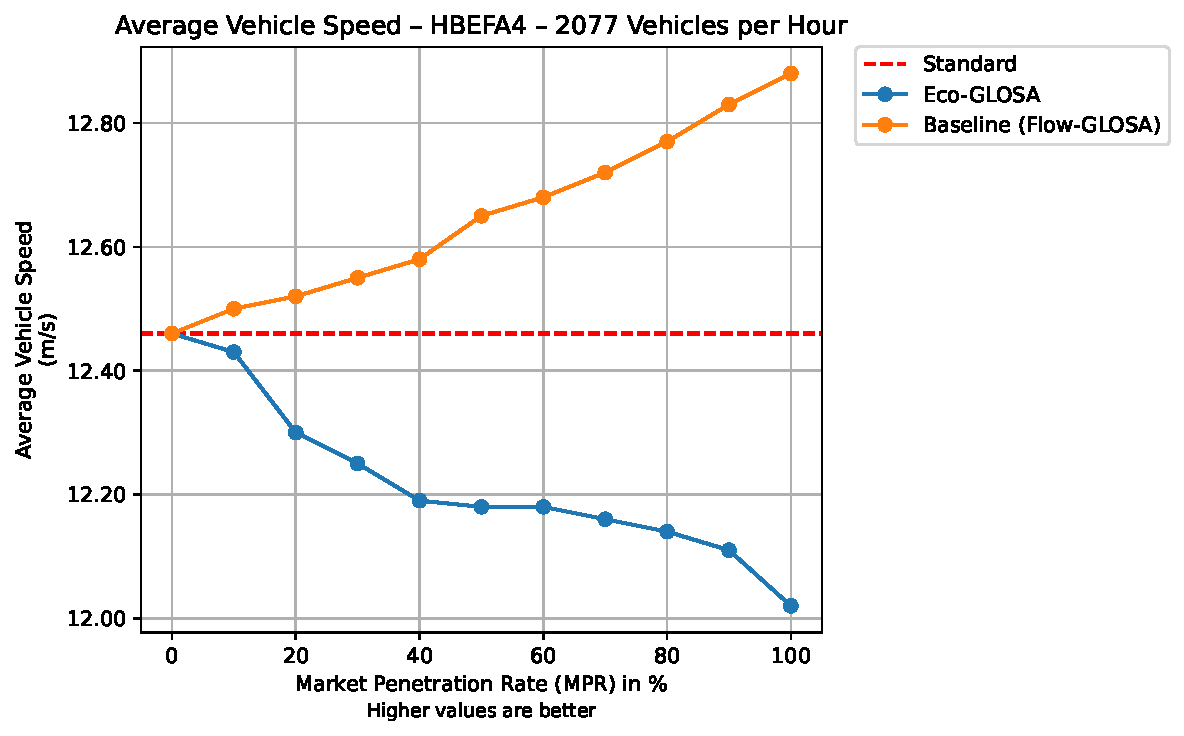
\includegraphics[width=\textwidth]{data/img/AverageVehicleSpeed/AverageVehicleSpeed_HBEFA4_Cars2077.pdf}
    \caption{Mean vehicle speed as a function of \ac{mpr} for the HBEFA4 emission model at a demand level of $2077\,\mathrm{veh/h}$.}
    \label{fig:MeanSpeed_HBEFA4_2077}
  \end{subfigure}\hfill
  \begin{subfigure}[b]{0.49\textwidth}
    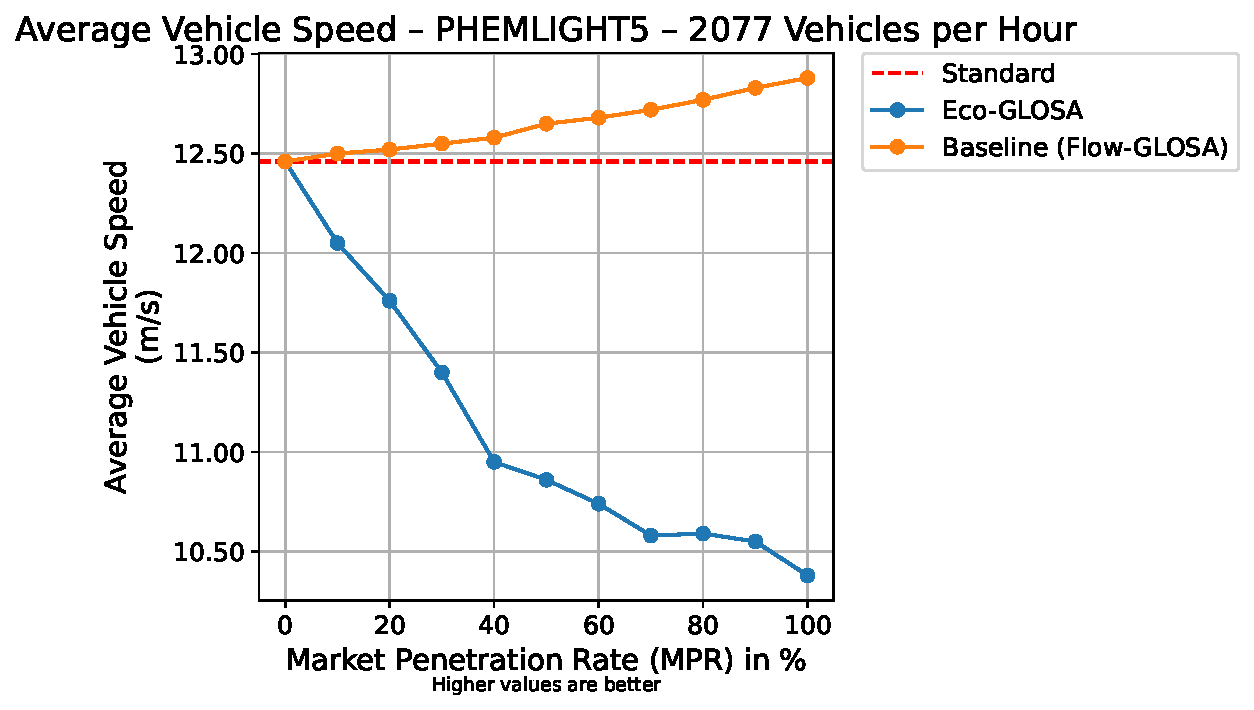
\includegraphics[width=\textwidth]{data/img/AverageVehicleSpeed/AverageVehicleSpeed_PHEMLIGHT5_Cars2077.pdf}
    \caption{Mean vehicle speed as a function of \ac{mpr} for the PHEMlight5 emission model at a demand level of $2077\,\mathrm{veh/h}$.}
    \label{fig:MeanSpeed_PHEM_2077}
  \end{subfigure}
  \caption{Mean vehicle speed as a function of \ac{mpr} at $2077\,\mathrm{veh/h}$ for the HBEFA4 and PHEMlight5 emission models. The plots show results for the Standard, \ac{eco-glosa}, and \ac{flow-glosa} algorithms.}
  \label{fig:MeanSpeed_2077}
\end{figure}


\begin{figure}[htb]
  \centering
  \begin{subfigure}[b]{0.49\textwidth}
    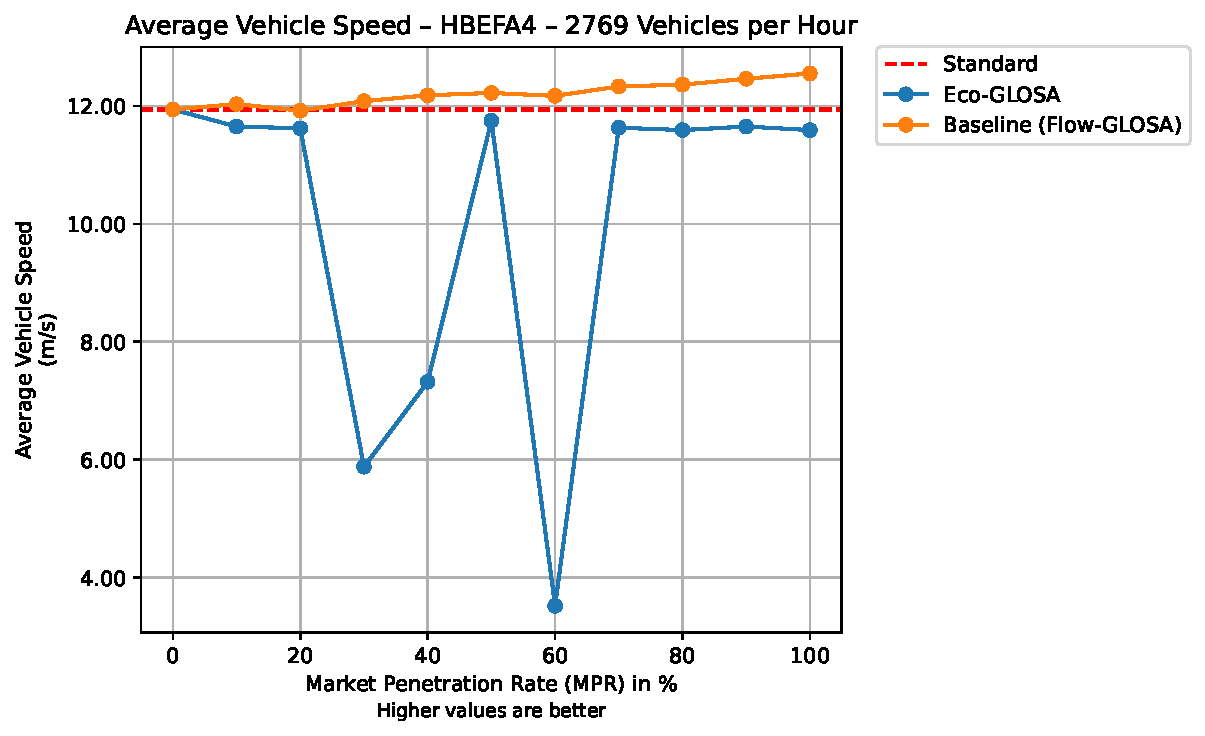
\includegraphics[width=\textwidth]{data/img/AverageVehicleSpeed/AverageVehicleSpeed_HBEFA4_Cars2769.pdf}
    \caption{Mean vehicle speed as a function of \ac{mpr} for the HBEFA4 emission model at $2769\,\mathrm{veh/h}$.}
    \label{fig:MeanSpeed_HBEFA4_2769}
  \end{subfigure}\hfill
  \begin{subfigure}[b]{0.49\textwidth}
    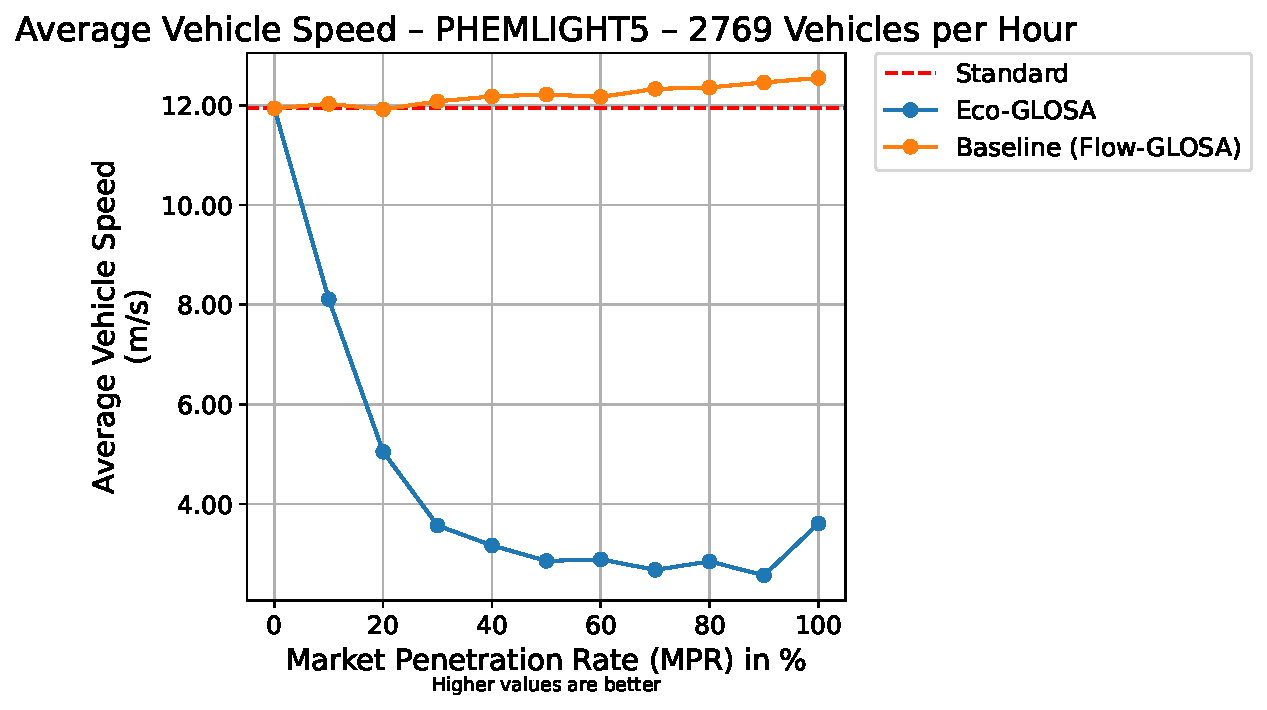
\includegraphics[width=\textwidth]{data/img/AverageVehicleSpeed/AverageVehicleSpeed_PHEMLIGHT5_Cars2769.pdf}
    \caption{Mean vehicle speed as a function of \ac{mpr} for the PHEMlight5 emission model at $2769\,\mathrm{veh/h}$.}
    \label{fig:MeanSpeed_PHEM_2769}
  \end{subfigure}
  \caption{Mean vehicle speed as a function of \ac{mpr} at $2769\,\mathrm{veh/h}$ for the HBEFA4 and PHEMlight5 emission models. The results include the Standard, \ac{eco-glosa}, and \ac{flow-glosa} algorithms.}
  \label{fig:MeanSpeed_2769}
\end{figure}

\begin{figure}[htb]
  \centering
  \begin{subfigure}[b]{0.49\textwidth}
    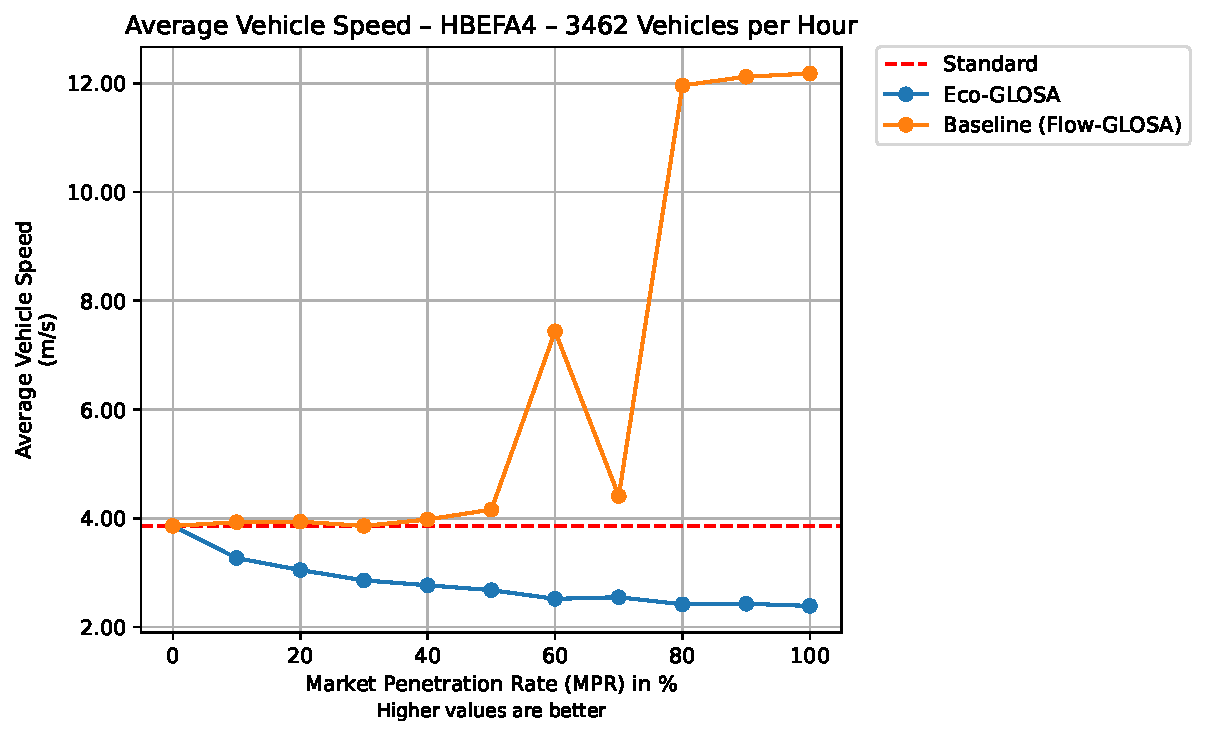
\includegraphics[width=\textwidth]{data/img/AverageVehicleSpeed/AverageVehicleSpeed_HBEFA4_Cars3462.pdf}
    \caption{Mean vehicle speed as a function of \ac{mpr} for the HBEFA4 emission model at $3462\,\mathrm{veh/h}$.}
    \label{fig:MeanSpeed_HBEFA4_3462}
  \end{subfigure}\hfill
  \begin{subfigure}[b]{0.49\textwidth}
    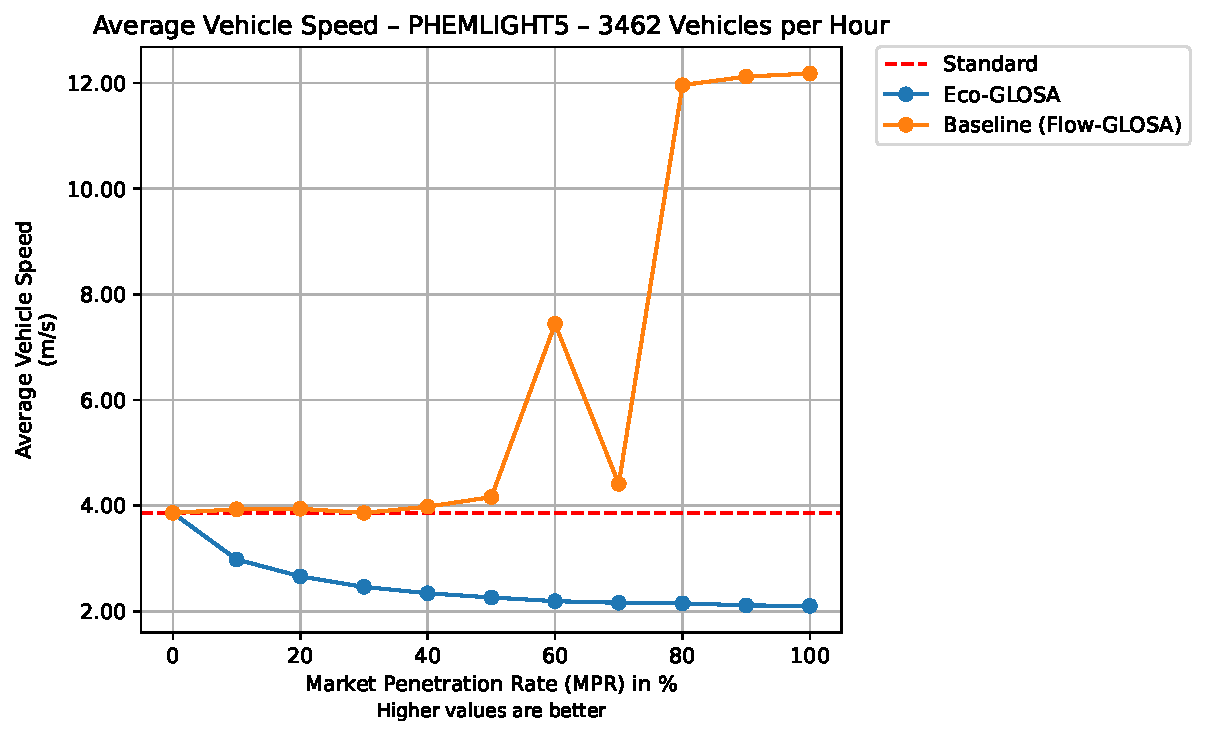
\includegraphics[width=\textwidth]{data/img/AverageVehicleSpeed/AverageVehicleSpeed_PHEMLIGHT5_Cars3462.pdf}
    \caption{Mean vehicle speed as a function of \ac{mpr} for the PHEMlight5 emission model at $3462\,\mathrm{veh/h}$.}
    \label{fig:MeanSpeed_PHEM_3462}
  \end{subfigure}
  \caption{Mean vehicle speed as a function of \ac{mpr} at $3462\,\mathrm{veh/h}$ for the HBEFA4 and PHEMlight5 emission models. The results are shown for the Standard, \ac{eco-glosa}, and \ac{flow-glosa} algorithms.}
  \label{fig:MeanSpeed_3462}
\end{figure}

\subparagraph*{Implications.}
\ac{flow-glosa}’s advisory logic is agnostic to the emission model, so its speed curves coincide exactly for HBEFA4 and PHEMLIGHT5 (see Figures~\ref{fig:MeanSpeed_HBEFA4_2077} and~\ref{fig:MeanSpeed_PHEM_2077}). By contrast, \ac{eco-glosa} computes its target speeds using the specific fuel model, yielding markedly different slowdowns: under PHEMLIGHT5 the mean speed at $2077\,\mathrm{veh/h}$ begins to fall at only $10\%$ \ac{mpr} (Figure~\ref{fig:MeanSpeed_PHEM_2077}), whereas under HBEFA4 the speed remains within $0.1\,\mathrm{m/s}$ of Standard until $30\%$ \ac{mpr} (Figure~\ref{fig:MeanSpeed_HBEFA4_2077}). Once the junction saturates ($3462\,\mathrm{veh/h}$), \ac{flow-glosa} can actually dissolve the queue at high \ac{mpr}, restoring free-flow speeds above $12\,\mathrm{m/s}$ (Figures~\ref{fig:MeanSpeed_HBEFA4_3462} and~\ref{fig:MeanSpeed_PHEM_3462}), whereas \ac{eco-glosa} remains gridlocked. At light to moderate volumes ($69$–$1385\,\mathrm{veh/h}$), \ac{eco-glosa} still offers marginal smoothing of stop-and-go oscillations, occasionally exceeding Standard by up to $0.04\,\mathrm{m/s}$ at $10\%$ \ac{mpr} (Figures~\ref{fig:MeanSpeed_HBEFA4_2077} and~\ref{fig:MeanSpeed_HBEM_2077}), but these gains vanish as \ac{mpr} exceeds $20\%$. Therefore, on lightly loaded arterials \ac{eco-glosa} may be deployed to fine-tune speed consistency, while on corridors operating near or above $2077\,\mathrm{veh/h}$ \ac{flow-glosa} is essential to maintain throughput, prevent premature queuing, and even resolve existing gridlock.

\begin{table}[htb]
  \centering
  \caption{Mean vehicle speed in meters per second ($\mathrm{m/s}$) as a function of traffic demand and \ac{mpr} for the different algorithm configurations. Outcomes are provided for the Baseline configuration (\ac{flow-glosa}), the Eco configuration (\ac{eco-glosa}), and the Standard case (no \ac{glosa}, $0\,\%$ \ac{mpr}).}
  \label{tab:MeanSpeed}
  \resizebox{\textwidth}{!}{%
  \begin{tabular}{r l l r *{10}{r}}
    \toprule
    Cars & Algorithm & Fuel & \textbf{0\% (Std)} & 10\% & 20\% & 30\% & 40\% & 50\% & 60\% & 70\% & 80\% & 90\% & 100\%\\
    \midrule
    69  & \ac{eco-glosa} & HBEFA4 & \textbf{13.34} & 13.86 & 13.45 & 13.71 & 13.51 & 13.46 & 13.71 & 13.72 & 13.05 & 13.81 & 13.01\\
    69  & Baseline (\ac{flow-glosa}) & HBEFA4 & \textbf{13.34} & 13.98 & 13.58 & 13.66 & 13.69 & 13.62 & 13.65 & 13.85 & 13.63 & 13.88 & 13.34\\
    69  & \ac{eco-glosa} & PHEMLIGHT5 & \textbf{13.34} & 13.89 & 13.38 & 13.79 & 13.60 & 12.77 & 13.30 & 13.23 & 12.81 & 13.70 & 12.34\\
    69  & Baseline (\ac{flow-glosa}) & PHEMLIGHT5 & \textbf{13.34} & 13.98 & 13.58 & 13.66 & 13.69 & 13.62 & 13.65 & 13.85 & 13.63 & 13.88 & 13.34\\
    \midrule
    138 & \ac{eco-glosa} & HBEFA4 & \textbf{13.24} & 13.51 & 13.29 & 13.46 & 13.56 & 13.36 & 13.52 & 13.17 & 13.12 & 13.01 & 12.97\\
    138 & Baseline (\ac{flow-glosa}) & HBEFA4 & \textbf{13.24} & 13.52 & 13.37 & 13.41 & 13.65 & 13.47 & 13.57 & 13.52 & 13.41 & 13.39 & 13.23\\
    138 & \ac{eco-glosa} & PHEMLIGHT5 & \textbf{13.24} & 13.38 & 13.40 & 13.36 & 13.64 & 13.15 & 13.39 & 13.03 & 12.99 & 12.70 & 12.50\\
    138 & Baseline (\ac{flow-glosa}) & PHEMLIGHT5 & \textbf{13.24} & 13.52 & 13.37 & 13.41 & 13.65 & 13.47 & 13.57 & 13.52 & 13.41 & 13.39 & 13.23\\
    \midrule
    346 & \ac{eco-glosa} & HBEFA4 & \textbf{13.24} & 13.24 & 13.14 & 13.07 & 13.18 & 13.01 & 13.08 & 13.04 & 12.96 & 12.99 & 12.87\\
    346 & Baseline (\ac{flow-glosa}) & HBEFA4 & \textbf{13.24} & 13.27 & 13.19 & 13.20 & 13.25 & 13.28 & 13.33 & 13.33 & 13.35 & 13.36 & \textbf{13.48}\\
    346 & \ac{eco-glosa} & PHEMLIGHT5 & \textbf{13.24} & 13.20 & 12.83 & 12.71 & 12.80 & 12.77 & 12.56 & 12.59 & 12.52 & 12.64 & 12.50\\
    346 & Baseline (\ac{flow-glosa}) & PHEMLIGHT5 & \textbf{13.24} & 13.27 & 13.19 & 13.20 & 13.25 & 13.28 & 13.33 & 13.33 & 13.35 & 13.36 & \textbf{13.48}\\
    \midrule
    692 & \ac{eco-glosa} & HBEFA4 & \textbf{13.17} & 13.13 & 13.17 & 13.09 & 13.04 & 13.01 & 13.05 & 12.94 & 12.91 & 12.82 & 12.81\\
    692 & Baseline (\ac{flow-glosa}) & HBEFA4 & \textbf{13.17} & 13.23 & 13.25 & 13.20 & 13.27 & 13.22 & 13.36 & 13.25 & 13.31 & 13.39 & 13.33\\
    692 & \ac{eco-glosa} & PHEMLIGHT5 & \textbf{13.17} & 13.08 & 12.95 & 12.71 & 12.68 & 12.52 & 12.49 & 12.38 & 12.24 & 12.11 & 12.10\\
    692 & Baseline (\ac{flow-glosa}) & PHEMLIGHT5 & \textbf{13.17} & 13.23 & 13.25 & 13.20 & 13.27 & 13.22 & 13.36 & 13.25 & 13.31 & 13.39 & 13.33\\
    \midrule
    1385 & \ac{eco-glosa} & HBEFA4 & \textbf{12.84} & 12.75 & 12.75 & 12.74 & 12.69 & 12.62 & 12.59 & 12.55 & 12.51 & 12.49 & 12.41\\
    1385 & Baseline (\ac{flow-glosa}) & HBEFA4 & \textbf{12.84} & 12.82 & 12.81 & 12.82 & 12.93 & 12.90 & 13.00 & 13.00 & 13.08 & 13.03 & 13.07\\
    1385 & \ac{eco-glosa} & PHEMLIGHT5 & \textbf{12.84} & 12.52 & 12.27 & 11.98 & 11.87 & 11.56 & 11.37 & 11.42 & 11.38 & 11.31 & 11.31\\
    1385 & Baseline (\ac{flow-glosa}) & PHEMLIGHT5 & \textbf{12.84} & 12.82 & 12.81 & 12.82 & 12.93 & 12.90 & 13.00 & 13.00 & 13.08 & 13.03 & 13.07\\
    \midrule
    2077 & \ac{eco-glosa} & HBEFA4 & \textbf{12.46} & 12.43 & 12.30 & 12.25 & 12.19 & 12.18 & 12.18 & 12.16 & 12.14 & 12.11 & 12.02\\
    2077 & Baseline (\ac{flow-glosa}) & HBEFA4 & \textbf{12.46} & 12.50 & 12.52 & 12.55 & 12.58 & 12.65 & 12.68 & 12.72 & 12.77 & 12.83 & 12.88\\
    2077 & \ac{eco-glosa} & PHEMLIGHT5 & \textbf{12.46} & 12.05 & 11.76 & 11.40 & 10.95 & 10.86 & 10.74 & 10.58 & 10.59 & 10.55 & 10.38\\
    2077 & Baseline (\ac{flow-glosa}) & PHEMLIGHT5 & \textbf{12.46} & 12.50 & 12.52 & 12.55 & 12.58 & 12.65 & 12.68 & 12.72 & 12.77 & 12.83 & 12.88\\
    \midrule
    2769 & \ac{eco-glosa} & HBEFA4 & \textbf{11.94} & 11.65 & 11.62 & \textbf{5.88} & \textbf{7.32} & 11.75 & \textbf{3.52} & 11.63 & 11.59 & 11.65 & 11.59\\
    2769 & Baseline (\ac{flow-glosa}) & HBEFA4 & \textbf{11.94} & 12.03 & 11.92 & 12.08 & 12.18 & 12.22 & 12.17 & 12.33 & 12.36 & 12.46 & 12.55\\
    \textbf{2769} & \textbf{\ac{eco-glosa}} & \textbf{PHEMLIGHT5} & \textbf{11.94} & \textbf{8.11} & \textbf{5.05} & \textbf{3.57} & \textbf{3.17} & \textbf{2.86} & \textbf{2.89} & \textbf{2.68} & \textbf{2.85} & \textbf{2.57} & \textbf{3.61}\\
    2769 & Baseline (\ac{flow-glosa}) & PHEMLIGHT5 & \textbf{11.94} & 12.03 & 11.92 & 12.08 & 12.18 & 12.22 & 12.17 & 12.33 & 12.36 & 12.46 & 12.55\\
    \midrule
    \textbf{3462} & \textbf{\ac{eco-glosa}} & \textbf{HBEFA4} & \textbf{3.86} & \textbf{3.27} & \textbf{3.05} & \textbf{2.86} & \textbf{2.77} & \textbf{2.68} & \textbf{2.52} & \textbf{2.55} & \textbf{2.42} & \textbf{2.43} & \textbf{2.39}\\
    3462 & Baseline (\ac{flow-glosa}) & HBEFA4 & \textbf{3.86} & 3.93 & 3.94 & 3.86 & 3.98 & 4.16 & \textbf{7.44} & 4.41 & \textbf{11.96} & \textbf{12.12} & \textbf{12.18}\\
    \textbf{3462} & \textbf{\ac{eco-glosa}} & \textbf{PHEMLIGHT5} & \textbf{3.86} & \textbf{2.98} & \textbf{2.66} & \textbf{2.46} & \textbf{2.34} & \textbf{2.26} & \textbf{2.19} & \textbf{2.16} & \textbf{2.15} & \textbf{2.11} & \textbf{2.10}\\
    3462 & Baseline (\ac{flow-glosa}) & PHEMLIGHT5 & \textbf{3.86} & 3.93 & 3.94 & 3.86 & 3.98 & 4.16 & \textbf{7.44} & 4.41 & \textbf{11.96} & \textbf{12.12} & \textbf{12.18}\\
    \bottomrule
  \end{tabular}
  }
\end{table}